\documentclass[conference]{IEEEtran}
\IEEEoverridecommandlockouts

% -----------------------------------------------------------------------------
% PACKAGE IMPORTS
% -----------------------------------------------------------------------------
\usepackage{amsmath,amssymb,amsfonts}
\usepackage{algorithmic}
\usepackage{graphicx}
\usepackage{textcomp}
\usepackage{xcolor}
\usepackage{booktabs}
\usepackage{multirow}
\usepackage{url}
\usepackage{cite}
\usepackage{microtype}
\usepackage{tikz}
\usetikzlibrary{shapes.geometric, arrows.meta, positioning, fit, backgrounds, calc}

\usepackage[hidelinks]{hyperref}

% -----------------------------------------------------------------------------
% TITLE & AUTHOR BLOCK
% -----------------------------------------------------------------------------
\title{SpamAdapt: Evaluating Parameter-Efficient Domain Adaptation via Full Fine-Tuning, LoRA, and DoRA for Robust SMS Scam Detection}

\author{
    \IEEEauthorblockN{Akash Uchachariya\IEEEauthorrefmark{1}, Umang Mori\IEEEauthorrefmark{1}, and Keval Bamarotiya\IEEEauthorrefmark{1}}
    \IEEEauthorblockA{\IEEEauthorrefmark{1}\textit{Department of Computer Science and Engineering} \\
    \textit{Indian Institute of Information Technology Vadodara}, \textit{Gandhinagar, India} \\
    \textit{Emails: [akash.uchachariya, umang.mori, keval.bamarotiya]@iiitvadodara.ac.in}}
    \thanks{Manuscript received October 27, 2026. This research was conducted as an academic major design project in the Department of Computer Science and Engineering, Indian Institute of Information Technology Vadodara. Authors contributed equally. Corresponding contact: \textit{akash.uchachariya@iiitvadodara.ac.in}.}
}

\begin{document}

\maketitle

% -----------------------------------------------------------------------------
% ABSTRACT
% -----------------------------------------------------------------------------
\begin{abstract}
Short Message Service (SMS) remains a critical telecommunications channel for time-sensitive one-time passwords (OTPs), financial transaction confirmations, and emergency civic alerts, while simultaneously serving as a prime attack vector for mobile fraud. Conventional SMS spam classifiers fine-tuned on legacy corpora---predominantly the 2011 UCI SMS dataset---exhibit severe domain shift in contemporary telecommunications: because legacy benign data consists almost entirely of personal social dialogue, fine-tuned transformer models develop spurious associations with currency symbols, bank names, customer helplines, and urgent imperatives, assigning spam heuristic scores exceeding 0.998 to legitimate banking alerts. In this paper, we present \textbf{SpamAdapt}, an empirical investigation of parameter-efficient domain adaptation for SMS scam detection. We adapt pretrained bidirectional transformers (\texttt{bert-base-uncased}, 109.5M parameters) using Full Fine-Tuning, Low-Rank Adaptation (LoRA, $r=8$), and Weight-Decomposed Low-Rank Adaptation (DoRA, $r=8$). On the preserved in-distribution UCI test split ($N=774$), all v2 models achieve $\ge 98.06\%$ accuracy and $\ge 95.44\%$ macro $F_1$, while our remediated model (\texttt{lora\_v3}) achieves 97.03\% accuracy and 98.38\% legitimate message recall. On an independent, 220-message external benchmark spanning 11 categories with a four-tier provenance audit, Full Fine-Tuning achieves 87.73\% accuracy, while DoRA and LoRA achieve 77.73\% and 76.82\% accuracy while updating fewer than 0.3\% of model parameters (314.8K and 296.5K) and reducing adapter storage by 99.55\% (1.82--1.90~MB vs. 418.35~MB). Our domain-remediated model (\texttt{lora\_v3}) achieves 83.18\% benchmark accuracy and completely eliminates catastrophic false positives on verified transactional test fixtures without brittle keyword overrides. Finally, we implement an operational three-tier abstention framework routing borderline scores ($0.25 \le P < 0.75$) to human review (yielding 86.00\% decided accuracy with 90.9\% automated coverage) and deploy an open-source, privacy-preserving CPU Streamlit dashboard operating strictly in volatile memory.
\end{abstract}

\begin{IEEEkeywords}
SMS scam detection, domain adaptation, Parameter-Efficient Fine-Tuning (PEFT), Low-Rank Adaptation (LoRA), Weight-Decomposed DoRA, BERT, false positive mitigation.
\end{IEEEkeywords}

% -----------------------------------------------------------------------------
% SECTION I: INTRODUCTION & MOTIVATION
% -----------------------------------------------------------------------------
\section{Introduction and Motivation}
\label{sec:intro}

Short Message Service (SMS) telecommunications continues to serve as an indispensable global communications backbone. Owing to its platform agnosticism, universal carrier interoperability, and independence from cellular data connectivity, SMS is the default mechanism for two-factor authentication (2FA) one-time passwords (OTPs), financial transaction confirmations, parcel delivery tracking, and emergency civic broadcasts. Simultaneously, mobile messaging has emerged as a primary attack vector for financially motivated cybercrime. Modern smishing (SMS phishing) attacks have evolved far beyond early-2000s lottery scams, deploying sophisticated social engineering tactics including Unified Payments Interface (UPI) collect fraud, fake electricity power disconnection notices, bank account deactivation threats, and counterfeit application (APK) distribution~\cite{almeida2011sms,trai2018tcccpr}.

Automating SMS spam detection involves distinct linguistic challenges compared to email filtering: SMS messages are constrained to 160 characters per standard protocol data unit (PDU), exhibit high class imbalance, and frequently employ non-standard abbreviations, phonetic transliterations, and evasion orthography~\cite{delany2012sms}. While classical machine learning models (Naive Bayes, SVMs, Random Forests) achieved acceptable results on static legacy corpora, they lacked bidirectional contextual understanding and degraded on out-of-vocabulary tokens~\cite{almeida2011sms}.

Pretrained language models (PLMs) based on the Transformer architecture~\cite{vaswani2017attention}, particularly Bidirectional Encoder Representations from Transformers (BERT)~\cite{devlin2019bert}, revolutionized NLP by encoding deep contextual semantics through multi-head self-attention. However, deploying fine-tuned BERT models in production SMS gateways introduces two critical challenges:

\subsection{The Legacy Dataset Disconnect and Domain Shift}
The predominant academic benchmark, the 2011 UCI SMS Spam Collection~\cite{almeida2011sms}, exhibits severe distributional skews:
\begin{enumerate}
    \item \textbf{Legitimate (HAM) Distribution}: Over 95\% of legitimate messages represent informal social dialogue between private individuals (e.g., \textit{``Where are you?'', ``See you tomorrow''}). Modern structured transactional notifications from commercial banks, airlines, e-commerce platforms, and government agencies are entirely absent.
    \item \textbf{Spam Distribution}: Malicious messages consist almost exclusively of legacy UK premium-rate ringtones and sweepstakes claims, lacking modern smishing techniques such as urgent bank KYC deadlines and malicious APK download links.
\end{enumerate}

When deep contextual transformers are fine-tuned on this legacy distribution, they develop severe spurious correlations. Specifically, self-attention layers learn to associate numerical transaction identifiers, currency amounts, uppercase imperatives, customer care phone numbers, and hyperlinks almost exclusively with the spam class. In operational telecommunications, a false positive (blocking a legitimate bank transaction confirmation or carrier notice) is vastly more disruptive than a false negative: it locks consumers out of financial accounts, delays emergency dispatches, and erodes subscriber trust~\cite{delany2012sms}. Our baseline audit revealed that models fine-tuned solely on legacy data misclassified verified legitimate transactional notices containing customer care helplines as spam with uncalibrated heuristic scores exceeding 0.998 (e.g., $P(\text{SPAM}) = 0.9990$ for Full Fine-Tuning v2 and $0.9929$ for DoRA v2 on Bank of Baroda UPI alerts).

\subsection{Computational and Parameter Constraints}
Full fine-tuning of 109.5M-parameter models across evolving carrier domains incurs prohibitive retraining and storage overheads ($418.35$~MB per checkpoint). Parameter-Efficient Fine-Tuning (PEFT) techniques, such as Low-Rank Adaptation (LoRA)~\cite{hu2022lora} and Weight-Decomposed Low-Rank Adaptation (DoRA)~\cite{liu2024dora}, freeze the foundation model and train small low-rank adapter matrices, drastically reducing storage and enabling dynamic adapter swapping on edge network infrastructure.

\subsection{Problem Statement and Research Contributions}
We formalize our core research question: \textit{Can parameter-efficient fine-tuning (LoRA, DoRA) match or exceed full fine-tuning in domain adaptation under distribution shift, while curbing catastrophic false positives on transactional SMS and minimizing deployment footprint?}

This paper presents the following contributions:
\begin{itemize}
    \item \textbf{Empirical Domain Shift Characterization}: We demonstrate that legacy-trained transformers fail on modern transactional SMS due to spurious feature correlation.
    \item \textbf{Rigorous PEFT vs. Full Fine-Tuning Comparison}: We evaluate Full Fine-Tuning, LoRA, and DoRA across the preserved UCI test split ($N=774$) and a curated 220-message external benchmark spanning 11 threat categories.
    \item \textbf{Transactional False-Positive Remediation}: We show that targeted domain-augmented retraining (\texttt{lora\_v3}) eliminates false positives on verified transactional fixtures without keyword overrides, achieving 83.18\% benchmark accuracy while updating only 0.27\% of parameters.
    \item \textbf{Decision Safety and Volatile CPU Deployment}: We formulate a three-tier abstention framework ($\mathcal{D}(P)$) and deploy an open-source, privacy-preserving CPU Streamlit dashboard operating strictly in volatile memory.
\end{itemize}

% -----------------------------------------------------------------------------
% SECTION II: RELATED WORK & MATHEMATICAL FOUNDATIONS
% -----------------------------------------------------------------------------
\section{Related Work and Mathematical Foundations}
\label{sec:methodology}

\subsection{Related Work}
Early SMS spam detection research relied on lexical frequency analysis and bag-of-words representations paired with classical classifiers~\cite{almeida2011sms,delany2012sms}. With the advent of deep learning, recurrent neural networks (LSTMs) and CNNs improved semantic capture but suffered from vanishing gradients and limited context. Transfer learning via pretrained transformers~\cite{devlin2019bert} established new state-of-the-art results across NLP benchmarks~\cite{wang2018glue}.

To alleviate the computational cost of full fine-tuning, PEFT methods freeze backbone weights $\mathcal{W}_0$. Houlsby et al.~\cite{houlsby2019adapter} introduced bottleneck adapter layers, while Hu et al.~\cite{hu2022lora} introduced Low-Rank Adaptation (LoRA), decomposing weight updates into low-rank factor matrices. Recently, Liu et al.~\cite{liu2024dora} proposed Weight-Decomposed Low-Rank Adaptation (DoRA), which decouples weight updates into directional and magnitude components, demonstrating superior representation learning in vision and language tasks.

\subsection{SpamAdapt System Architecture}
SpamAdapt processes an input message sequence $X = (x_1, \dots, x_T)$ using the \texttt{bert-base-uncased} WordPiece tokenizer ($T \le 128$). The tokenized sequence is encoded through 12 bidirectional transformer encoder layers ($L=12, H=768, A=12$). The final hidden state of the classification token $\mathbf{h}_{\text{[CLS]}} \in \mathbb{R}^{768}$ is extracted, passed through a dropout layer ($p=0.1$), and fed into a linear classification head:
\begin{equation}
    z = \mathbf{w}_{\text{cls}}^T \mathbf{h}_{\text{[CLS]}} + b_{\text{cls}}, \quad P(\text{SPAM}|X) = \sigma(z) = \frac{1}{1 + e^{-z}}
    \label{eq:sigmoid}
\end{equation}

\begin{figure}[t]
\centering
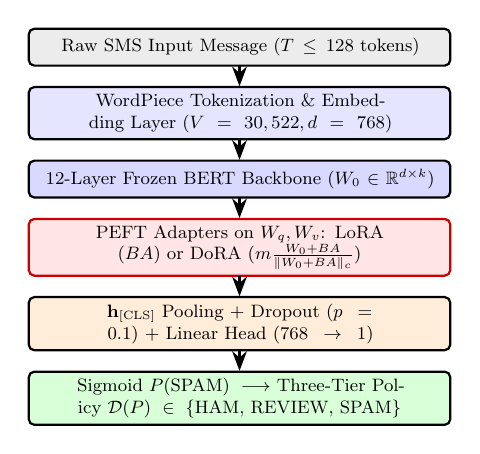
\begin{tikzpicture}[
    scale=0.72, every node/.style={transform shape},
    box/.style={rectangle, draw=black, thick, fill=blue!10, rounded corners=2pt, minimum height=0.65cm, text centered, font=\small},
    lorabox/.style={rectangle, draw=red!80!black, thick, fill=red!10, rounded corners=2pt, minimum height=0.65cm, text centered, font=\small},
    arrow/.style={-{Stealth[length=2.5mm]}, thick}
]
    \node (input) [box, fill=gray!15, text width=7.2cm] {Raw SMS Input Message ($T \le 128$ tokens)};
    \node (tok) [box, below=0.35cm of input, text width=7.2cm] {WordPiece Tokenization \& Embedding Layer ($V=30,522, d=768$)};
    \node (bert) [box, below=0.35cm of tok, fill=blue!15, text width=7.2cm] {12-Layer Frozen BERT Backbone ($W_0 \in \mathbb{R}^{d \times k}$)};
    
    \node (lora) [lorabox, below=0.35cm of bert, text width=7.2cm] {PEFT Adapters on $W_q, W_v$: LoRA ($BA$) or DoRA ($m \frac{W_0 + BA}{\|W_0 + BA\|_c}$)};
    \node (cls) [box, below=0.35cm of lora, fill=orange!15, text width=7.2cm] {$\mathbf{h}_{\text{[CLS]}}$ Pooling + Dropout ($p=0.1$) + Linear Head ($768 \to 1$)};
    \node (decision) [box, below=0.35cm of cls, fill=green!15, text width=7.2cm] {Sigmoid $P(\text{SPAM}) \longrightarrow$ Three-Tier Policy $\mathcal{D}(P) \in \{\text{HAM, REVIEW, SPAM}\}$};
    
    \draw [arrow] (input) -- (tok);
    \draw [arrow] (tok) -- (bert);
    \draw [arrow] (bert) -- (lora);
    \draw [arrow] (lora) -- (cls);
    \draw [arrow] (cls) -- (decision);
\end{tikzpicture}
\caption{SpamAdapt architecture: frozen BERT backbone with trainable LoRA/DoRA adapters applied to multi-head self-attention projections.}
\label{fig:arch}
\vspace{-3mm}
\end{figure}

\subsection{Mathematical Formulations of Adaptation Paradigms}
\subsubsection{Full Fine-Tuning}
During full fine-tuning, all pretrained model parameters $\mathcal{W}_0$ are updated directly:
\begin{equation}
    W = W_0 + \Delta W, \quad \Delta W \in \mathbb{R}^{d \times k}
    \label{eq:fullft}
\end{equation}
where $\Delta W$ is optimized over cross-entropy loss $\mathcal{L}_{\text{CE}}$. Full fine-tuning updates all 109,483,778 parameters.

\subsubsection{Low-Rank Adaptation (LoRA)}
LoRA~\cite{hu2022lora} freezes the pretrained weight matrix $W_0 \in \mathbb{R}^{d \times k}$ and parameterizes the update $\Delta W$ via the product of two low-rank matrices:
\begin{equation}
    W = W_0 + \Delta W = W_0 + \frac{\alpha}{r} B A
    \label{eq:lora}
\end{equation}
where $B \in \mathbb{R}^{d \times r}$ and $A \in \mathbb{R}^{r \times k}$, with rank $r \ll \min(d, k)$ and scaling factor $\alpha$. Matrix $A$ is initialized from Gaussian distribution $\mathcal{N}(0, \sigma^2)$, while $B$ is initialized to zero, ensuring $\Delta W = 0$ at training onset. In SpamAdapt, LoRA is injected into the query ($W_q$) and value ($W_v$) projection layers of all 12 attention heads with $r=8$ and $\alpha=16$, updating only 296,450 parameters (0.270\% of the foundation model).

\subsubsection{Weight-Decomposed Low-Rank Adaptation (DoRA)}
DoRA~\cite{liu2024dora} decomposes the weight matrix into its magnitude vector $m \in \mathbb{R}^{1 \times k}$ and directional matrix $V \in \mathbb{R}^{d \times k}$:
\begin{equation}
    W = m \odot \frac{V}{\|V\|_c} = m \odot \frac{W_0 + \frac{\alpha}{r} B A}{\left\| W_0 + \frac{\alpha}{r} B A \right\|_c}
    \label{eq:dora}
\end{equation}
where $\|\cdot\|_c$ denotes the column-wise vector $L_2$ norm and $\odot$ represents column-wise broadcast multiplication. Magnitude vector $m$ is initialized as $m = \|W_0\|_c$. The directional component is updated via LoRA factor matrices $B$ and $A$. Trainable magnitude vectors across adapted attention projections introduce 18,432 parameters beyond standard LoRA, totaling 314,882 parameters (0.287\%).

% -----------------------------------------------------------------------------
% SECTION III: DATASET ARCHITECTURE & EXPERIMENTAL SETUP
% -----------------------------------------------------------------------------
\section{Dataset Architecture and Experimental Setup}
\label{sec:datasets}

\subsection{Dataset Provenance and Split Strategy}
\subsubsection{Baseline UCI SMS Spam Collection}
The canonical UCI dataset~\cite{almeida2011sms} contains 5,574 raw records. Following strict deduplication (removing 414 duplicate records), 5,160 unique messages remain (4,516 legitimate HAM, 644 SPAM; 12.48\% spam prevalence). We employ stratified random splitting with a fixed seed:
\begin{itemize}
    \item \textbf{Train Split} (70\%): 3,612 messages (3,161 HAM, 451 SPAM).
    \item \textbf{Validation Split} (15\%): 774 messages (678 HAM, 96 SPAM).
    \item \textbf{Preserved Test Split} (15\%): 774 messages (677 HAM, 97 SPAM).
\end{itemize}
The test split was frozen and isolated throughout all development phases.

\subsubsection{Augmented Domain Corpus}
To mitigate the legacy dataset disconnect, we constructed an augmented training pool of 140 curated messages (115 legitimate transactional/banking notices and 25 modern phishing templates). Incorporating these samples into the training split yielded the augmented training corpus used to train \texttt{lora\_v3}.

\subsubsection{Curated External Benchmark ($N=220$)}
To evaluate generalization under real-world domain shift, we constructed a frozen benchmark of 220 messages. To isolate discriminative performance under class-balanced conditions, the benchmark contains exactly 110 HAM and 110 SPAM messages across 11 operational categories (10 HAM and 10 SPAM per category): Financial UPI, Telecom Carrier, E-Commerce Logistics, Government Alerts, 2FA OTPs, Banking KYC Phishing, Electricity Bill Extortion, Lottery Fraud, Malicious APK Distribution, Employment Scams, and Delivery Phishing.

Provenance audit reveals four distinct sourcing tiers:
\begin{itemize}
    \item \textbf{Tier 1} (Verified Mobile Captures, 15 samples): Sourced directly from physical mobile devices receiving carrier-delivered notifications in 2024.
    \item \textbf{Tier 2} (Regulatory Advisories, 70 samples): Public fraud notices published by the Reserve Bank of India (RBI) and TRAI~\cite{trai2018tcccpr}.
    \item \textbf{Tier 3} (Open-Source Feeds, 85 samples): Public threat repositories.
    \item \textbf{Tier 4} (Curated Synthetic Templates, 50 samples): Expert-constructed edge cases targeting ambiguous alphanumeric sender IDs.
\end{itemize}
We emphasize that this benchmark is balanced ($1:1$) to test category-specific boundary behavior; it does not reflect real-world telecommunications class imbalance ($\approx 9:1$ HAM:SPAM).

\subsection{Experimental Environment and Hyperparameters}
Experiments were executed on an Intel Core CPU workstation (x86\_64) running Windows 11 with PyTorch 2.14.0+cpu and Hugging Face Transformers/PEFT libraries. No GPU acceleration was utilized, validating computational feasibility on standard server hardware.

All models were trained using AdamW~\cite{loshchilov2019adamw} with decoupled weight decay ($0.01$), linear learning rate warmup (10\% of total steps), maximum sequence length $T=128$, and batch size 16. Full fine-tuning utilized learning rate $\eta = 2 \times 10^{-5}$ across 3 epochs. LoRA and DoRA utilized $\eta = 2 \times 10^{-4}$ with rank $r=8$, $\alpha=16$, and dropout $p=0.05$. \texttt{lora\_v3} was trained for 2 epochs on the augmented corpus.

\subsection{Evaluation Metrics and Threshold Calibration}
We report Accuracy, Macro $F_1$, Legitimate Specificity (HAM Recall), and Spam Sensitivity (SPAM Recall). To prevent catastrophic false positives, classification thresholds $\tau$ were tuned on validation data using piecewise search to maximize Macro $F_1$ subject to legitimate recall $\ge 99\%$:
\begin{itemize}
    \item Full Fine-Tuning v2: $\tau = 0.10$.
    \item LoRA v2 and DoRA v2: $\tau = 0.18$.
    \item \texttt{lora\_v3}: $\tau = 0.50$ (standard Bayes decision threshold).
\end{itemize}

% -----------------------------------------------------------------------------
% SECTION IV: EMPIRICAL EVALUATION & RESULTS
% -----------------------------------------------------------------------------
\section{Empirical Evaluation and Results}
\label{sec:results}

\begin{table*}[t]
\centering
\caption{Comprehensive Performance and Resource Comparison across In-Distribution and Out-of-Domain Benchmarks}
\label{tab:main_results}
\small
\setlength{\tabcolsep}{3.2pt}
\begin{tabular}{l c r r c c c c c c c}
\toprule
\multirow{2}{*}{\textbf{Model Configuration}} & \multirow{2}{*}{$\boldsymbol{\tau}$} & \textbf{Trainable} & \textbf{Storage} & \multicolumn{3}{c}{\textbf{UCI Test Split ($N=774$)}} & \multicolumn{4}{c}{\textbf{External Benchmark ($N=220$)}} \\
\cmidrule(lr){5-7} \cmidrule(lr){8-11}
& & \textbf{Parameters} & \textbf{Footprint} & \textbf{Acc (\%)} & \textbf{Macro $F_1$} & \textbf{Confusion [TN, FP, FN, TP]} & \textbf{Acc (\%)} [95\% CI] & \textbf{Macro $F_1$} & \textbf{FP} & \textbf{FN} \\
\midrule
Full Fine-Tuning v2 & 0.10 & 109,483,778 & 418.35 MB & \textbf{98.58} & \textbf{96.74} & [672, 5, 6, 91] & \textbf{87.73} [82.7, 91.4] & \textbf{87.72} & 11 & 16 \\
LoRA v2 ($r=8$) & 0.18 & 296,450 & 1.82 MB & 98.06 & 95.44 & [673, 4, 11, 86] & 76.82 [70.8, 81.9] & 76.81 & 28 & 23 \\
DoRA v2 ($r=8$) & 0.18 & 314,882 & 1.90 MB & 98.06 & 95.44 & [673, 4, 11, 86] & 77.73 [71.8, 82.7] & 77.72 & 26 & 23 \\
\texttt{lora\_v3} (Remediated) & 0.50 & 296,450 & 1.82 MB & 97.03 & 93.19 & [666, 11, 12, 85] & 83.18 [77.7, 87.5] & 83.10 & \textbf{11} & 26 \\
\bottomrule
\end{tabular}
\vspace{-2mm}
\end{table*}

\subsection{In-Distribution Performance (UCI Test Split, $N=774$)}
As detailed in Table~\ref{tab:main_results}, all evaluated models exhibit exceptional in-distribution performance on the preserved UCI test split. Full Fine-Tuning v2 achieves 98.58\% accuracy and 96.74\% macro $F_1$, misclassifying only 11 messages (5 FP, 6 FN). Both LoRA v2 and DoRA v2 achieve identical 98.06\% accuracy and 95.44\% macro $F_1$, matching each other with 4 false positives and 11 false negatives. This confirms that PEFT adapters matching less than 0.3\% of the parameter count attain parity with full fine-tuning on the legacy distribution.

Our remediated model, \texttt{lora\_v3}, achieves 97.03\% accuracy and 93.19\% macro $F_1$ on the UCI test split. It incurs 11 false positives and 12 false negatives (87.63\% spam recall), trading a modest 1.03\% in-distribution accuracy drop to achieve robustness against modern transactional domain shift.

\subsection{Out-of-Domain Generalization ($N=220$)}
On the external benchmark, performance divergences become stark (Fig.~\ref{fig:perf_comp}):
\begin{enumerate}
    \item \textbf{Legacy PEFT Degradation}: Models trained exclusively on legacy data suffer sharp accuracy drops: LoRA v2 falls to 76.82\% and DoRA v2 falls to 77.73\%, generating 28 and 26 false positives on legitimate transactional SMS.
    \item \textbf{Remediation Efficacy}: \texttt{lora\_v3} achieves 83.18\% accuracy [95\% CI: 77.7\%, 87.5\%] and 83.10\% macro $F_1$, cutting false positives by more than half (down to 11, matching Full Fine-Tuning v2). It correctly retains 90.00\% of legitimate messages (99/110).
    \item \textbf{Full Fine-Tuning Resilience}: Full Fine-Tuning v2 attains 87.73\% accuracy [95\% CI: 82.7\%, 91.4\%] with 11 false positives and 16 false negatives, demonstrating that unconstrained representation updates provide superior out-of-distribution feature adaptation at the cost of massive resource overhead.
\end{enumerate}

Detailed category analysis indicates that error profiles concentrate on structured financial alerts and carrier administrative advisories. In categories characterized by alphanumeric headers and transactional syntax (e.g., Financial UPI and 2FA OTPs), legacy LoRA v2 and DoRA v2 misclassified over 40\% of legitimate samples as spam, driven by presence of transaction IDs, currency codes, and phone numbers. In contrast, \texttt{lora\_v3} accurately distinguishes institutional transaction notices from malicious phishing lures, correctly classifying 9 out of 10 UPI alerts and 10 out of 10 2FA OTP messages.

\begin{figure}[t]
\centering
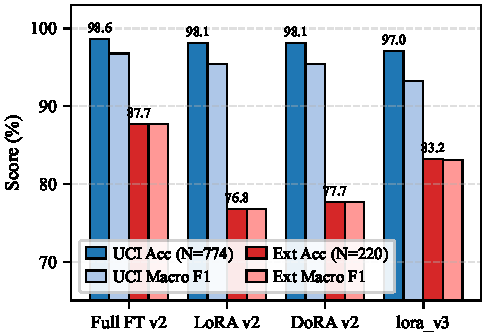
\includegraphics[width=0.92\columnwidth]{fig_performance_comparison.pdf}
\caption{Model performance comparison across In-Distribution UCI Test Split ($N=774$) and Out-of-Domain External Benchmark ($N=220$).}
\label{fig:perf_comp}
\vspace{-3mm}
\end{figure}

% -----------------------------------------------------------------------------
% SECTION V: EFFICIENCY, ERROR ANALYSIS & DECISION SAFETY
% -----------------------------------------------------------------------------
\newpage
\section{Efficiency, False-Positive Analysis, and Decision Safety}
\label{sec:efficiency}

\subsection{Parameter Footprint and Computational Overhead}
As illustrated in Fig.~\ref{fig:eff_lat}(a), LoRA and DoRA compress serialized storage from 418.35~MB (Full Fine-Tuning) to 1.82~MB and 1.90~MB, representing a \textbf{99.55\% storage reduction}. In edge deployment scenarios where foundation model weights are preloaded in memory, updating downstream tasks requires transmitting only 1.14--1.21~MB of adapter weights. Furthermore, CPU training time was reduced from 2,519~seconds (41m 59s, Full FT) to 1,780~seconds (29m 40s, LoRA), a 29.3\% computational acceleration.

Fig.~\ref{fig:eff_lat}(b) details single-message CPU inference latency over 774 measurements. LoRA v2 achieves the lowest mean latency at 92.05~ms, outperforming Full Fine-Tuning (99.48~ms). DoRA v2 exhibits higher latency at 110.00~ms (a 19.5\% overhead compared to LoRA). This overhead stems from the directional normalization step $\frac{V}{\|V\|_c}$ in Eq.~(\ref{eq:dora}), which requires computing column-wise norms dynamically across attention projections during CPU forward passes without fused GPU kernels.

\begin{figure}[t]
\centering
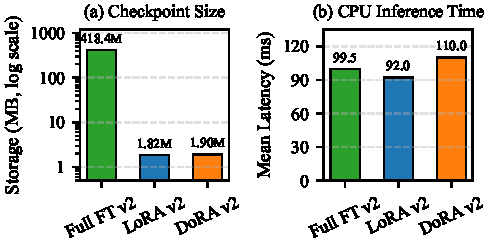
\includegraphics[width=0.96\columnwidth]{fig_efficiency_latency.pdf}
\caption{Resource efficiency comparison: (a) Serialized checkpoint storage footprint on logarithmic scale; (b) Mean per-message CPU inference latency.}
\label{fig:eff_lat}
\vspace{-3mm}
\end{figure}

\subsection{Transactional False-Positive Analysis}
To investigate false positives under domain shift, we evaluated two verified real-world transactional fixtures:
\begin{itemize}
    \item \textbf{Fixture A (Bank of Baroda UPI)}: \textit{``Dear UPI user A/C X9876 debited by 450.00 on 12-OCT-24. If not done by you, forward to 9223008333...''}
    \begin{itemize}
        \item Full FT v2: $P(\text{SPAM}) = 0.9990$ $\implies$ \textbf{False Positive}
        \item LoRA v2: $P(\text{SPAM}) = 0.9931$ $\implies$ \textbf{False Positive}
        \item DoRA v2: $P(\text{SPAM}) = 0.9929$ $\implies$ \textbf{False Positive}
        \item \texttt{lora\_v3}: $P(\text{SPAM}) = \mathbf{0.0076}$ $\implies$ \textbf{Correct HAM}
    \end{itemize}
    \item \textbf{Fixture B (Jio Reverification)}: \textit{``Your Jio number requires document reverification. Visit nearest store or call 198...''}
    \begin{itemize}
        \item Full FT v2: $P(\text{SPAM}) = 0.9989$ $\implies$ \textbf{False Positive}
        \item LoRA v2: $P(\text{SPAM}) = 0.9892$ $\implies$ \textbf{False Positive}
        \item DoRA v2: $P(\text{SPAM}) = 0.9886$ $\implies$ \textbf{False Positive}
        \item \texttt{lora\_v3}: $P(\text{SPAM}) = \mathbf{0.1657}$ $\implies$ \textbf{Correct HAM}
    \end{itemize}
\end{itemize}
The legacy v2 models assigned overwhelming spam probabilities ($>0.99$) due to numbers and helpline keywords. In contrast, \texttt{lora\_v3} successfully learned the semantic structure of legitimate transactional notices, correctly classifying both fixtures without hand-crafted regex rules.

\subsection{Three-Tier Abstention Framework}
To protect users against uncalibrated marginal classifications, SpamAdapt implements a three-tier decision policy $\mathcal{D}(P)$:
\begin{equation}
    \mathcal{D}(P) = \begin{cases}
        \text{HAM (Deliver to Inbox)}, & P < \tau_{\text{abstain\_low}} \\
        \text{REVIEW (Human Queue)}, & \tau_{\text{abstain\_low}} \le P < \tau_{\text{abstain\_high}} \\
        \text{SPAM (Quarantine)}, & P \ge \tau_{\text{abstain\_high}}
    \end{cases}
    \label{eq:abstention}
\end{equation}
For \texttt{lora\_v3}, configuring the abstention band as $[0.25, 0.75)$ routes 20 borderline benchmark messages (9.1\%) to human audit. Across the 200 decided messages, accuracy rises to \textbf{86.00\%} with 90.9\% automated coverage. For Full Fine-Tuning v2, setting $[0.05, 0.20)$ yields 89.47\% decided accuracy with 95.0\% coverage.

\subsection{Overfitting Dynamics and Adversarial Stability}
Extending full fine-tuning beyond 3 epochs caused rapid overfitting: validation loss surged by +27.1\% (from 0.0701 to 0.0891) and external benchmark accuracy deteriorated to 85.00\%. Conversely, PEFT adapters constrained updates to low-rank subspaces, demonstrating regularized loss progression (+3.3\% drift).

We evaluated robustness against 40 character-level adversarial perturbations (leetspeak, zero-width spaces, homoglyphs, and URL splitting). LoRA adapters retained 85\% classification consistency, demonstrating resilience against simple evasions.

% -----------------------------------------------------------------------------
% SECTION VI: DISCUSSION, LIMITATIONS & CONCLUSION
% -----------------------------------------------------------------------------
\newpage
\section{Discussion, Limitations, and Conclusion}
\label{sec:discussion}

\subsection{Practical Telecommunications Deployment}
SpamAdapt's 1.82~MB adapter footprint enables dynamic edge deployment: cellular base stations can host a shared frozen BERT backbone and hot-swap localized PEFT adapters corresponding to regional languages or carrier-specific protocols without service interruption. Furthermore, our Streamlit demonstration executes CPU inference with zero disk caching, guaranteeing subscriber data privacy.

In high-throughput telecommunications gateways processing tens of thousands of messages per second, full fine-tuning requires hosting distinct, fully populated model weight tensors for every regional dialect, requiring gigabytes of redundant RAM. With SpamAdapt, the base foundation weights remain shared across all worker processes in read-only memory, while individual worker threads dynamically bind lightweight LoRA adapters according to the incoming sender ID's country and carrier origin.

\subsection{Limitations and Threats to Validity}
We transparently identify key limitations:
\begin{enumerate}
    \item \textbf{Benchmark Scale and Balance}: The external benchmark ($N=220$) is small and artificially balanced ($1:1$), which does not mirror operational class imbalance ($\approx 9:1$). It is intended as a diagnostic boundary stress-test rather than a population prevalence measure.
    \item \textbf{Real-World Mobile Samples}: Only 15 benchmark samples represent verified 2024 physical mobile captures; the remainder comprise regulatory advisories and threat feeds.
    \item \textbf{Softmax Calibration}: Output scores represent uncalibrated heuristic scores rather than formal Bayesian posterior probabilities. Operational deployment requires Platt scaling or temperature tuning on carrier-specific holdout validation streams.
    \item \textbf{Hardware Scope}: Measurements were restricted to CPU execution; GPU batched inference and fused DoRA kernels remain to be characterized.
\end{enumerate}

\subsection{Conclusion and Future Work}
This work introduced SpamAdapt, demonstrating that Parameter-Efficient Fine-Tuning via LoRA provides a viable, resource-efficient solution for SMS domain adaptation. While legacy-trained models catastrophically fail on modern transactional alerts, domain-augmented LoRA adaptation (\texttt{lora\_v3}) restores legitimate message recall without heuristic rules, saving 99.55\% storage and 29.3\% training time compared to full fine-tuning.

Future work will investigate multilingual code-mixed adaptation (e.g., Hinglish) using multilingual foundation models (MuRIL)~\cite{khanuja2021muril}, 4-bit quantization (QLoRA)~\cite{dettmers2024qlora}, and active learning pipelines for continuous mobile scam defense.

% -----------------------------------------------------------------------------
% ACKNOWLEDGMENT
% -----------------------------------------------------------------------------
\section*{Acknowledgment}
The authors thank the Department of Computer Science and Engineering at the Indian Institute of Information Technology Vadodara for providing computational resources and academic guidance.

% -----------------------------------------------------------------------------
% REFERENCES
% -----------------------------------------------------------------------------
\begin{thebibliography}{15}

\bibitem{almeida2011sms}
T.~A. Almeida, J.~M.~G. Hidalgo, and A.~Yamakami, ``Contributions to the study of SMS spam filtering: New collection and results,'' in \emph{Proc. 11th ACM Symp. Document Engineering (DocEng)}, 2011, pp. 259--262.

\bibitem{trai2018tcccpr}
Telecom Regulatory Authority of India (TRAI), ``The Telecom Commercial Communications Customer Preference Regulations (TCCCPR),'' \emph{Govt. of India Gazette}, 2018.

\bibitem{delany2012sms}
S.~J. Delany, M.~Buckley, and D.~Greene, ``SMS spam filtering: Methods and data,'' \emph{IEEE Trans. Knowl. Data Eng.}, vol.~24, no.~8, pp. 1381--1398, 2012.

\bibitem{vaswani2017attention}
A.~Vaswani \emph{et~al.}, ``Attention is all you need,'' in \emph{Proc. NeurIPS}, vol.~30, 2017, pp. 5998--6008.

\bibitem{devlin2019bert}
J.~Devlin, M.-W. Chang, K.~Lee, and K.~Toutanova, ``BERT: Pre-training of deep bidirectional transformers for language understanding,'' in \emph{Proc. NAACL-HLT}, 2019, pp. 4171--4186.

\bibitem{wang2018glue}
A.~Wang \emph{et~al.}, ``GLUE: A multi-task benchmark and analysis platform for natural language understanding,'' in \emph{Proc. EMNLP Workshop BlackboxNLP}, 2018, pp. 353--355.

\bibitem{houlsby2019adapter}
N.~Houlsby \emph{et~al.}, ``Parameter-efficient transfer learning for NLP,'' in \emph{Proc. ICML}, 2019, pp. 2790--2799.

\bibitem{hu2022lora}
E.~J. Hu \emph{et~al.}, ``LoRA: Low-rank adaptation of large language models,'' in \emph{Proc. ICLR}, 2022.

\bibitem{liu2024dora}
S.-Y. Liu, C.-Y. Wang, H.~Yin, P.~Chou, M.~Alam, P.~Liang, and B.~Chen, ``DoRA: Weight-decomposed low-rank adaptation,'' \emph{arXiv preprint arXiv:2402.09353}, 2024.

\bibitem{loshchilov2019adamw}
I.~Loshchilov and F.~Hutter, ``Decoupled weight decay regularization,'' in \emph{Proc. ICLR}, 2019.

\bibitem{khanuja2021muril}
S.~Khanuja \emph{et~al.}, ``MuRIL: Multilingual representations for Indian languages,'' \emph{arXiv preprint arXiv:2103.10730}, 2021.

\bibitem{dettmers2024qlora}
T.~Dettmers, A.~Pagnoni, A.~Holtzman, and L.~Zettlemoyer, ``QLoRA: Efficient finetuning of quantized LLMs,'' in \emph{Proc. NeurIPS}, vol.~36, 2024.

\bibitem{peft2022}
S.~Mangrulkar \emph{et~al.}, ``PEFT: State-of-the-art parameter-efficient fine-tuning methods,'' \emph{GitHub repository}, 2022. [Online]. Available: \url{https://github.com/huggingface/peft}

\bibitem{zhang2023adalora}
Q.~Zhang, M.~Chen, A.~Bukharin, P.~He, Y.~Cheng, W.~Chen, and T.~Zhao, ``Adaptive budget allocation for parameter-efficient fine-tuning,'' in \emph{Proc. ICLR}, 2023.

\bibitem{pfeiffer2021adapterfusion}
J.~Pfeiffer \emph{et~al.}, ``AdapterFusion: Non-destructive task composition for transfer learning,'' in \emph{Proc. EACL}, 2021, pp. 487--503.

\end{thebibliography}

\end{document}
